
\documentclass[a4paper,12pt]{article}
%%%%%%%%%%%%%%%%%%%%%%%%%%%%%%%%%%%%%%%%%%%%%%%%%%%%%%%%%%%%%%%%%%%%%%%%%%%%%%%%%%%%%%%%%%%%%%%%%%%%%%%%%%%%%%%%%%%%%%%%%%%%%%%%%%%%%%%%%%%%%%%%%%%%%%%%%%%%%%%%%%%%%%%%%%%%%%%%%%%%%%%%%%%%%%%%%%%%%%%%%%%%%%%%%%%%%%%%%%%%%%%%%%%%%%%%%%%%%%%%%%%%%%%%%%%%
\usepackage{eurosym}
\usepackage{vmargin}
\usepackage{amsmath}
\usepackage{graphics}
\usepackage{epsfig}
\usepackage{framed}
\usepackage{subfigure}
\usepackage{fancyhdr}
\usepackage{framed}
\usepackage{subfiles}
\usepackage{graphics}
\usepackage{newlfont}
\usepackage{eurosym}
\usepackage{amsmath,amsthm,amsfonts}
\usepackage{amsmath}
\usepackage{enumerate}
\usepackage{color}
\usepackage{multicol}
\usepackage{amssymb}
\usepackage{multicol}
\usepackage[dvipsnames]{xcolor}
\usepackage{graphicx}

\setcounter{MaxMatrixCols}{10}
%TCIDATA{OutputFilter=LATEX.DLL}
%TCIDATA{Version=5.00.0.2570}
%TCIDATA{<META NAME="SaveForMode"CONTENT="1">}
%TCIDATA{LastRevised=Wednesday, February 23, 201113:24:34}
%TCIDATA{<META NAME="GraphicsSave" CONTENT="32">}
%TCIDATA{Language=American English}

\pagestyle{fancy}
\setmarginsrb{20mm}{0mm}{20mm}{25mm}{12mm}{11mm}{0mm}{11mm}
\lhead{MA4128} \rhead{Kevin O'Brien} \chead{Binary Classification} %\input{tcilatex}

%http://www.electronics.dit.ie/staff/ysemenova/Opto2/CO_IntroLab.pdf
\begin{document}



\section*{ROC Curves}
\begin{itemize}
	\item  A receiver operating characteristic (ROC), or ROC curve, is a graphical plot that illustrates
	the performance of a binary classification system as its discrimination threshold is varied.
	\item  The ROC curve is created by plotting the true positive rate against the false positive rate at
	various threshold settings. (The true-positive rate is also known as sensitivity in biomedicine,
	or recall in machine learning. The false-positive rate is also known as the fall-out and can be
	calculated as 1 - specificity).

\end{itemize}
%====================================================%
\begin{itemize}
	\item In statistics, a receiver operating characteristic (ROC), or ROC curve, is a graphical plot that illustrates the performance of a binary classifier system as its discrimination threshold is varied. The curve is created by plotting the true positive rate against the false positive rate at various threshold settings. (The true-positive rate is also known as sensitivity in biomedicine, or recall in machine learning. The false-positive rate is also known as the fall-out and can be calculated as 1 - specificity). 
	
	\item The ROC curve is thus the sensitivity as a function of fall-out. In general, if the probability distributions for both detection and false alarm are known, the ROC curve can be generated by plotting the cumulative distribution function (area under the probability distribution from $-\infty$ to $+\infty$) of the detection probability in the y-axis versus the cumulative distribution function of the false-alarm probability in x-axis.
	
	\item ROC analysis provides tools to select possibly optimal models and to discard suboptimal ones independently from (and prior to specifying) the cost context or the class distribution. ROC analysis is related in a direct and natural way to cost/benefit analysis of diagnostic decision making.
	
	\item The ROC curve was first developed by electrical engineers and radar engineers during World War II for detecting enemy objects in battlefields and was soon introduced to psychology to account for perceptual detection of stimuli. ROC analysis since then has been used in medicine, radiology, biometrics, and other areas for many decades and is increasingly used in machine learning and data mining research.
	

	\item The ROC is also known as a relative operating characteristic curve, because it is a comparison of two operating characteristics (TPR and FPR) as the criterion changes.








%\subsection*{Receiver Operating Characteristic (ROC) curve}
%\begin{figure}
%	\centering
%	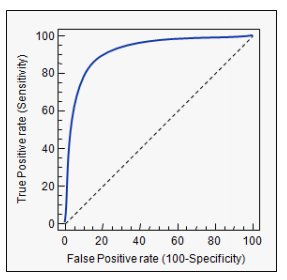
\includegraphics[width=0.55\linewidth]{ROCcurve}
%	\caption{}
%	\label{fig:roccurve}
%\end{figure}

\end{itemize}

\begin{figure}[h!]
	\centering
	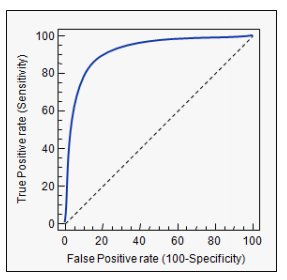
\includegraphics[width=0.7\linewidth]{ROCcurve}
	\caption{}
	\label{fig:roccurve}
\end{figure}


\begin{itemize}
	\item In a Receiver Operating Characteristic (ROC) curve the true positive rate
	(Sensitivity) is plotted in function of the false positive rate (100-Specificity)
	for different cut-off points. 
	\item Each point on the ROC curve represents a sensitivity/specificity
	pair corresponding to a particular decision threshold. 
	\item A
	test with perfect discrimination (no overlap in the two distributions) has a
	ROC curve that passes through the upper left corner (100\% sensitivity, 100\%
	specificity). 
	\item Therefore the closer the ROC curve is to the upper left corner,
	the higher the overall accuracy of the test. %(Zweig and Campbell, 1993).
\end{itemize}




%----------------------------------------------------------------------------------%
\subsection*{Properties of ROC Curves}
% ROC Curves
% Specificity and Sensitivity
An ROC curve demonstrates several things:
\begin{enumerate}
	\item It shows the tradeoff between sensitivity and specificity (any increase in sensitivity will be accompanied by a decrease in specificity).
	\item The closer the curve follows the upper-left border of the ROC space, the more accurate the test.
	\item The closer the curve comes to the 45-degree diagonal of the ROC space, the less accurate the test.
	\item The slope of the tangent line at a cutpoint gives the likelihood ratio (LR) for that value of the test.
	\item The area under the curve is a measure of accuracy.
\end{enumerate}


\end{document}
